\documentclass[../thesis/thesis.tex]{subfiles}
\begin{document}

\chapter{Design}
\label{chap:design}

In this chapter, we explain the methodology used to fill the research gap identified in Chapter~\ref{chap:litreview}, thereby producing a system that identifies high-potential startup companies that are likely to receive additional funding or a exit in a given forecast window. Figure~\ref{fig:design:system_architecture} depicts the system architecture, which we describe in detail in the following sections.

\begin{figure}[!htb]
    \centering
    \includegraphics[width=\textwidth]{../figures/design/system_architecture}
    \caption{System architecture overview.}
    \label{fig:design:system_architecture}
\end{figure}

\begin{enumerate}

\item Data Collection. We collected startup company data from the CrunchBase online database, with supplementation from PatentsView. We collected two CSV dumps from CrunchBase in September 2016 and April 2017, for training and testing respectively. We imported these CSV files into a relational database (SQLite) and performed aggregation queries to create features suitable for classification. We then performed screening based on each company's developmental stage and age to ensure only relevant companies were included in the dataset. Finally, we explored the dataset and identified issues of sparsity, long-tailed distributions, imbalanced feature ranges, and non-orthogonality.

\item Pipeline Creation. In the previous step, we identified a range of issues with our dataset. In this step, we develop a processing pipeline that seeks to address these issues and produce accurate predictions. Our pipeline is developed using the popular Python-based machine learning library Scikit-learn \cite{pedregosa2011}. Pre-processing steps include imputation, transformation, scaling and extraction. Each pre-processing step has hyperparameters that can be tuned (e.g. imputation strategy, number of components to extract) that affect its performance. We also tested a number of common classification algorithms and their hyperparameters. We performed a randomised search across the pipeline's hyperparameters to generate a selection of candidate pipelines. The hyperparameters that had the most significant effect on the final performance of the pipelines were related to the classification algorithms.

\item Pipeline Selection. In the previous step, we generated a cross-section of candidate pipelines with different hyperparameters. In this step, we rank these candidate pipelines and test the best pipelines (finalist pipelines) over a number of different dataset slices. This process ensures that we select pipelines that are robust in their performance with respect to time. We aggregate the results for each finalist pipeline across these dataset slices and rank the finalist pipelines on their overall performance. Finally, we select the best pipeline.

%TODO - What is the variance in performance over time in aggregate?
%TODO - What is the variance over time between different classifiers?
%TODO - How many finalists do we need to ensure we get the best pipeline?

\item Pipeline Evaluation. In the previous step, we selected the best pipeline with respect to the robustness of its performance over time. In this step, we evaluate the best pipeline's performance on a held-out test dataset. We use the pipeline to fit a model to a dataset sliced from the master database. We apply this model to another feature vector from the master database and make predictions. We score these predictions against truth values derived from the held-out test database (c. Apr-17). This process is performed multiple times to evaluate our three primary criteria: efficiency, robustness, and predictive power. The experiments are as follows: efficiency, the pipeline is fitted to datasets of various sample sizes; robustness, the pipeline is fitted to datasets from various time slices; and predictive power, the forecast window between the feature vector and outcome is varied. Results of these experiments are described in detail in Chapter~\ref{chap:evaluation}.

\end{enumerate}

\section{Data Collection}

In the previous chapter, we reviewed the literature concerning data sources for entrepreneurship and \gls{vc} investment. We concluded the most promising primary data sources for this project are CrunchBase and AngelList, for their size, comprehensiveness and ease of access. We suggested PatentsView (the online database of the US Patent Office) could be a useful secondary data source for structural capital features. In the following sections, we first discuss how we collected data from CrunchBase and PatentsView, converted the relational databases into a format suitable for machine learning, performed preliminary screening to ensure we only included relevant companies. This process is depicted in Figure~\ref{fig:design:data_collection}. Following our description of this process we describe the results of exploratory analysis on our dataset and identify dataset issues which will be addressed in later steps.

\begin{figure}[!htb]
    \centering
    \includegraphics[width=\textwidth]{../figures/design/data_collection}
    \caption{Data collection overview.}
    \label{fig:design:data_collection}
\end{figure}

\subsection{CrunchBase}

CrunchBase is an online, crowd-sourced repository of startup companies, individuals and investors with a focus on US high-tech sectors. CrunchBase is freely accessible for browsing but requires licenses to filter the dataset, use the API, and download Microsoft Excel and CSV-formatted dumps. For the purposes of this project, we were granted an Academic License. CrunchBase provides database access in a few formats that offer trade-offs in terms of accessibility and comprehensiveness. We intended to use CrunchBase's API because it provides the most comprehensive access to their database. We developed a collector that downloaded a daily list of updated API endpoints from CrunchBase and queried nodes it needed to update. CrunchBase's API provides JSON-formatted responses which the program recursively parsed and stored into a relational database. However, due to the time constraints of this research project, we abandoned this data collection method. CrunchBase also provides CSV-formatted dumps of their key endpoints (e.g. organizations, people, funding rounds). We downloaded two CSV-formatted dumps from Crunchbase on 09 September 2016 and 04 April 2017 which we loaded into relational databases (see Appendix~\ref{appendix:database_schema} for the full database schema).

\subsection{PatentsView}

In 2015, the \gls{uspto} launched PatentsView, a free public API to allow programmatic access to their database. PatentsView holds over 12 million patent filings from 1976 onwards \cite{schultz2016}. The database provides comprehensive information on patents, their inventors, their organisations, and locations. We collected the patent filing records of each company in the primary database, focusing on information relating to dates, citations, and patent types. We matched the data sources on standardised company names (removing common suffixes, punctuation etc.) and using normalised Levenshtein distances. Although approximate matching introduces error, the volume of companies in the database is too high to be matched manually and there are no other identifying records. We stored the PatentsView data in a relation which we merged into our master and test databases.

\subsection{Dataset Preparation}

To prepare the dataset for machine learning, we first flattened the relational database into a single file using SQL aggregation queries. We aggregated each relevant relation in turn, grouping by Company ID and then combined each aggregated table using left outer joins. Following this process, we used Python to convert tuples (e.g. Round Type and Round Date) and lists (e.g. Round Types) into dummy variables.

We performed preliminary screening on the primary dataset (N = 425,934) to ensure it only included relevant companies. We were interested in removing traditional, non-startup businesses from the dataset (e.g. consulting firms, companies that will not take \gls{vc} funding etc.). To do this, we explored two factors for each company: developmental stage and age. By developmental stage, we primarily refer to external funding milestones. These stages are associated with shifts in a startup company's functions and objectives and we also expect them to correlate with company age. Our dataset as grouped by startup developmental stage is depicted in Figure~\ref{fig:design:lifecycle}.

\begin{figure}[!htb]
    \centering
    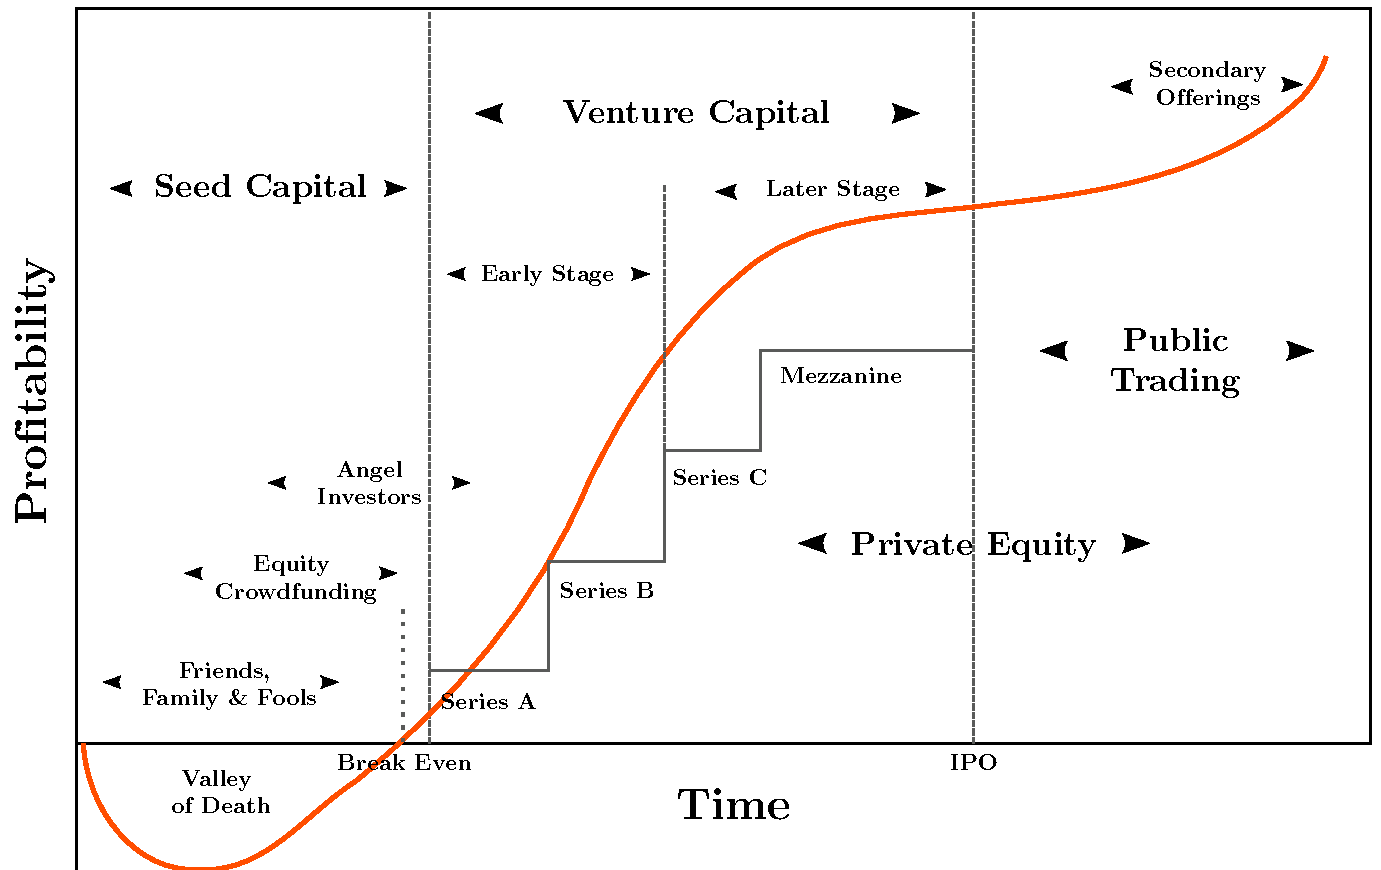
\includegraphics[width=\textwidth]{../figures/design/lifecycle}
    \caption{Idealised startup development lifecycle (adapted, \cite{}) with company counts from the master dataset (c. September 2016). Red line represents profitability over time. The chart is divided into three periods: an early period of unprofitability (``Valley of Death'') where seed capital supports the business, a period of growth sustained by rounds of venture capital, and a transition to stability and mature capital markets.}
    \label{fig:design:lifecycle}
\end{figure}

After attempting to place the companies into development stages we are left with a large group of companies (the majority of the dataset) that have not raised funding and so can not be classified on that basis. We assume that companies that have not raised funding fall into two groups - those that intend to raise funding but have not had time to yet, and those that have chosen not to pursue funding and are unlikely to do so. We separated these groups by applying a cutoff equal to the 90th percentile of the age of companies in the Seed category, and excluded the older group from further analyses (N = 227,162,  53.3\%). As we are only interested in companies that could theoretically seek investment, we also excluded Closed, Acquired and IPO groups from further analyses (N = 35,973, 8.4\%).

Figure\ref{fig:design:stages_ages} depicts the ages of companies in the master dataset, grouped by developmental stage.  As we expected, there is a strong relationship between company stage and company age. Most pre-Series A companies are under five years old, and the majority of Series D+ funded companies are under 10 years old and the 75th percentile is at 15 years old. On this basis, we excluded companies that are over the 75th percentile of the age of companies in the Series D+ category (N =9,756, 2.2\%). Overall, our preliminary screening steps reduced the dataset from 425,934 companies to 153,043 companies, a reduction of 64.1\%.

\begin{figure}[!htb]
    \centering
    \includegraphics[width=\textwidth]{../figures/design/stages_ages}
    \caption{Company ages in years grouped by developmental stage. While there is significant variability in age for each developmental stage, there is a broad positive relationship between age and developmental stage. The dashed blue line represents the 75th percentile of the age of companies in the Series D+ category (15.7 years).}
    \label{fig:design:stages_ages}
\end{figure}

\subsection{Exploratory Analysis}

\subsubsection{Descriptive Statistics}

Table~\ref{} presents the descriptive statistics for the dataset. The dataset is heavily skewed towards New companies (i.e. companies that were recently founded and have not raised any type of funding yet, 84.8\%). The interquartile ranges imply significant variability in all measures.

%INCLUDE DESCRIPTIVE STATS TABLE - waiting for patents data

CrunchBase's approach to industry classification is simplistic compared to other classification schemes (e.g., USSIC, NAICS, VentureSource) which generally have an industry hierarchy with tiers for broad industry sectors and sub-sectors providing further granularity. As a result, CrunchBase class labels include over represented and vague classes (e.g., ``Software'', ``Internet Services'') which could describe the majority of companies included in the database. In fact, ``Software'' and ``Internet Services'' account for 16.4\% and 13.4\% of all companies in the dataset respectively (see Figure~\ref{fig:design:industry_counts}). Despite these vague class labels, it is clear the dataset skews towards high technology startups, as opposed to biomedical, agricultural, or other technologies.

\begin{figure}[!htb]
    \centering
    \includegraphics[width=\textwidth]{../figures/design/industry_counts}
    \caption{Companies grouped by industry sector. The 10 most common sectors are displayed. Source: Master dataset (c. September 2016).}
    \label{fig:design:industry_counts}
\end{figure}

\subsubsection{Sparsity}

First, we explored missing data in the dataset. We expected the dataset to be highly sparse because it primarily came from CrunchBase, a crowd-sourced database. As profiles are entered into CrunchBase piece-meal, it is not clear at face-value whether data (e.g. records of funding rounds) is missing or didn't occur. Figure~\ref{fig:design:sparsity} displays the distribution of missing data in the dataset, with respect to each feature and each feature. The multi-modal peaks of both distributions suggest that missing data across certain groups of features may be correlated with each other (e.g. all features derived from funding rounds).

\begin{figure}[!htb]
    \centering
    \begin{subfigure}{\textwidth}
        \includegraphics[width=\textwidth]{../figures/design/sparsity_features}
        \caption{Distribution of missing data by company}
        \label{fig:design:sparsity:features}
    \end{subfigure}
    \begin{subfigure}{\textwidth}
        \includegraphics[width=\textwidth]{../figures/design/sparsity_observations}
        \caption{Distribution of missing data by feature}
        \label{fig:design:sparsity:observations}
    \end{subfigure}
    \caption{Distribution of missing data in master dataset (c. September 2016).}
    \label{fig:design:sparsity}
\end{figure}

\subsubsection{Normality}

Next, we explored the distributions of features. As we identified in the last section, the dataset is highly sparse. %TODO -

\begin{figure}[!htb]
    \centering
    \begin{subfigure}{\textwidth}
        \includegraphics[width=\textwidth]{../figures/design/skew}
        \caption{Distribution of skew by feature}
        \label{fig:design:normality:skew}
    \end{subfigure}
    \begin{subfigure}{\textwidth}
        \includegraphics[width=\textwidth]{../figures/design/kurtosis}
        \caption{Distribution of kurtosis by feature}
        \label{fig:design:normality:kurtosis}
    \end{subfigure}
    \caption{Distribution of features in master dataset (c. September 2016).}
    \label{fig:design:normality}
\end{figure}

\subsubsection{Scale}

%TODO - write para

\begin{figure}[!htb]
    \centering
    \includegraphics[width=\textwidth]{../figures/design/scaling}
    \caption{Distribution of interquartile ranges (transformed by log1p) in master dataset (c. September 2016).}
    \label{fig:design:scaling}
\end{figure}

\subsubsection{Orthogonality}

%TODO - write para

\begin{figure}[!htb]
    \centering
    \includegraphics[width=\textwidth]{../figures/design/orthogonality}
    \caption{Distribution of intercorrelations in master dataset (c. September 2016).}
    \label{fig:design:orthogonality}
\end{figure}

\section{Pipeline Creation}

We developed a classification pipeline using the popular Python-based machine learning library Scikit-learn \cite{pedregosa2011}. The classification pipeline construct allows us to easily search across hyperparameters at each step in the pipeline (see Appendix~\ref{appendix:pipeline_hyperparameters} for hyperparameter list). The following sections explore the testing of each hyperparameter decision, and the selection of primary classifiers for the following steps. This process is depicted in Figure~\ref{fig:design:pipeline_creation}.

\begin{figure}[!htb]
    \centering
    \includegraphics[width=\textwidth]{../figures/design/pipeline_creation}
    \caption{Pipeline creation overview.}
    \label{fig:design:pipeline_creation}
\end{figure}

\subsection{Imputation}

After reviewing the distribution of missing data, we decided to perform further investigation into imputation methods. Common imputation strategies include replacing missing values with the mean, median or mode of each feature. Figure~\ref{} shows the distribution of mean, median and modes for each feature in the dataset. For the majority of features, all three measures of central tendency are equal to zero. This resolves the issue of distinguishing missing data from negative observations because, following imputation, all of these data points will map to zero. Figure~\ref{} shows the receiver-operating characteristics of the different imputation strategies. As expected, all three imputation strategies produce similar results (within the margin of error).

\begin{figure}[!htb]
    \centering
    \includegraphics[width=\textwidth]{../figures/design/central_tendency}
    \caption{Distribution of measures of central tendency (mean, median and mode) in master dataset (c. September 2016).}
    \label{fig:design:central_tendency}
\end{figure}

%INCLUDE ROC curve for imputer strategies

\subsection{Transformation}

While the classification algorithms we identified in the previous chapter are relatively robust to violations of normality, it may be beneficial to transform the data if the feature distributions are extreme. Figure~\ref{} shows one of the key features, Total Funding Raised, under a number of different transformations. Like many features in our dataset, the distribution of Total Funding Raised is highly skewed. The log transformation reduces this skew (a normal distribution of non-zero values is apparent) and square root transformation also reduces this skew (to a lesser extent). The impact of these transformations is reduced by the extent of their zero-inflation. However, it is still reasonable to expect both of these transformations to improve the classification accuracy. Figure~\ref{} shows the \gls{roc} of these different transformation functions. Both functions provide a small performance improvement, with the square root function narrowly best.

%INCLUDE Funding under different transformations

%INCLUDE ROC curve for transformation strategies

\subsection{Scaling}

Standardisation of datasets is a common requirement for many feature extraction methods and machine learning estimators. Sci-kit learn provides three primary scaling functions: StandardScaler, RobustScaler and MinMaxScaler. RobustScaler is intended to alleviate the effect of outliers while MinMaxScaler is intended to preserve zero entries in sparse data - both of these are relevant properties for the dataset. Figure~\ref{} shows the receiver-operating characteristics of the different scaling functions. MinMaxScaler and RobustScaler actually underperform the null condition while StandardScaler only performs on par with the null condition. This is unexpected but may be caused by the previously applied transformations.

%INCLUDE ROC curve for scaling strategies

\subsection{Extraction}

Feature extraction reduces high-dimensional data into lower-dimensional data in such a way that maximises the variance of the data. The most common approach to dimensionality reduction is \gls{pca}, which constructs orthogonal eigenvectors (components). The magnitude of each eigenvector (its eigenvalue) is displayed in Figure~\ref{}. The majority of explained variance is captured in the first 10 components, and the Eigenvalues drop below 1 by 100 components - this suggests that these are reasonable values for further hyperparameter search. Figure~\ref{} shows the \gls{roc} for different numbers of extracted components. All curves produce similar classification results (within margin of error) which implies that we should extract between 1 - 20 components (Group 0) because it will provide us with more efficient computation.

%INCLUDE PCA scree plot

%INCLUDE ROC curve for extraction strategies

While PCA is efficient at reducing features, the resultant components are not interpretable. Similarly, individual analysis of 400\+ features is difficult to interpret. A compromise is to group the features using the conceptual framework we developed earlier from the literature review. The grouping approach applied weights to each individual feature that optimised the inter-correlations within each group. Given the highly skewed features, we use Spearman correlation which is robust to skewness because it is based on ranking. Figure~\ref{} displays the inter-correlations between each factor from the proposed conceptual framework. As we would expect, 'investors' and 'funding' features are highly correlated. While 'investors' attempts to capture the influence of previous investors, it also captures features like the size of an investor's past investments, which would likely correlate with the size of the investment they made in the target company. Interestingly, 'founders' features are positively correlated with all other features except for 'advisors' features which are negatively correlated with all other feature groups.

%INCLUDE Grouped inter-correlation matrix

\subsection{Classification Algorithms}

The literature review we performed in the previous chapter revealed seven common supervised classification algorithms potentially suitable for application to this problem area. Our review suggested that Random Forests were most likely to provide a successful trade-off between predictive power, interpretability and time taken. We empirically tested each of these classifiers and compared their performance against a range of metrics, as displayed in Table~\ref{}. We made our comparisons based on maximum recorded scores rather than measures of central tendency to ensure we didn't penalise algorithms that had unfavourable hyperparameter search spaces. The classifiers receiver operating characteristics are showed in Figure~\ref{}.

%INCLUDE Classification accuracy metrics

%INCLUDE ROC curve for each algorithm

%INCLUDE learning curve at creation - grouped by algorithm

\subsection{Conclusion}

%TODO

\section{Pipeline Selection}

%TODO - section preamble

\begin{figure}[!htb]
    \centering
    \includegraphics[width=\textwidth]{../figures/design/pipeline_selection}
    \caption{Pipeline selection overview.}
    \label{fig:design:pipeline_selection}
\end{figure}

%TODO - What is the variance in performance over time in aggregate?
%TODO - What is the variance over time between different classifiers?
%TODO - How many finalists do we need to ensure we get the best pipeline?

%INCLUDE Learning curve at selection - grouped by training slice

The best candidate pipeline is depicted in Table~\ref{}. We adopted this pipeline configuration for the following experiments.

%INCLUDE Hyperparameters of our final classification pipeline

\section{Pipeline Evaluation}

%TODO - section preamble

\begin{figure}[!htb]
    \centering
    \includegraphics[width=\textwidth]{../figures/design/pipeline_evaluation}
    \caption{Pipeline evaluation overview.}
    \label{fig:design:pipeline_evaluation}
\end{figure}

\subsection{Efficiency}

A rationale for this research project is the need for more efficient forms of \gls{vc} investment analysis which leverage technology, particularly in surfacing and screening. By its nature, our automated system should be more efficient than current manual methods but it's also important to determine how to most efficiently use the data that we have. For these reasons, we decided to investigate the learning curves for our classification pipeline to determine whether we could use smaller samples from our dataset to achieve similar predictive power and reduce our need for computational power and time taken. We used cross-validation to split our dataset 10 times and used subsets of the training set with varying sizes to train the estimator and produce training and test scores for each subset size. The convergence or divergence of our training and cross-validation curves will imply whether our classification pipeline is over- or under-fitting our data for various sizes allowing us to select an optimal sample size.

\subsection{Robustness}

It is critical that our system be robust with respect to time so investors can rely on its future predictions based on historical models. CrunchBase provides created and last-updated timestamps for each record in their CSV-formatted dumps (and also in the JSON-formatted responses from their API). We took advantage of this to produce a system that  reverse-engineers previous database states by filtering the current database by only records that were created by a given 'slice' date. We performed preliminary testing of this technique by comparing a historical CrunchBase database collected in December 2013 with a slice from our primary dataset collected in September 2016, as shown in Table~\ref{}. While there are some differences in the records, particularly in the IPO relation, we consider this to be satisfactory variance considering the 3-year time period. The key relations for our purposes are Companies, Funding Rounds and People, all of which had minor differences considering the size of these datasets. Table~\ref{} shows company counts by startup development stage from different dataset slices. We limited our experiments to dataset slices from 2012-onwards because prior to 2012 the datasets become too small to use to make predictions (given the class imbalance).

%INCLUDE - Comparison of 2013 slice from 2016 dataset

%INCLUDE - Counts of observations from dataset slices of various ages


\subsection{Predictive Power}

Finally, we test our system's predictive power for making forecasts of different time periods. We use the same system of reverse-engineering time slices that we used in our previous experiment to robustness, but this time we vary the time difference between the slice that provides our features and the slice that provides our label. Preliminary testing on a April 2013 features slice collected from the September 2016 is shown in Table 3.7. Very few companies appear to change stage over a period of less than 2 years so we will focus our experimentation on forecast windows of 2-4 years. We performed testing against labels from the April 2017 dataset.

%INCLUDE - Counts of merged observations from dataset slices of various ages

%INCLUDE - Proportion of companies increased in development stage


\ifcsdef{mainfile}{}{\printbibliography}
\end{document}
